\chapter{Architecture}

Overall, system architecture is shown in Figure~\ref{fig:architecture}. Apart from the HIP-VPLS switches
we have also implemented special control-plane protocol on top of the SSL protocol. According to the 
protocol, on one hand, every HIP-VPLS switch reports to the central controller (and authenticated using HMAC algorithm
together with the shared symmetric master secret). On the other hand, every HIP-VPLS switches obtains the configuration
from the central controller (such as mesh configuration, HIT resolver information, firewall rules and MAC-based ACL).
In the future, we also plan to support traffic shaper functionality.

%In our architecture, HIP switch controller is a central server instance that collects information from the HIP-switches
%and allows one to perform configuration of such parameters as firewall rules, HIP hosts file, MAC-based access
%controll lists (ACL) and configure traffic shaper. We are going to discuss each feature seperately 
%in the proceeding paragraphs.  

\begin{figure}[h!]
\centering
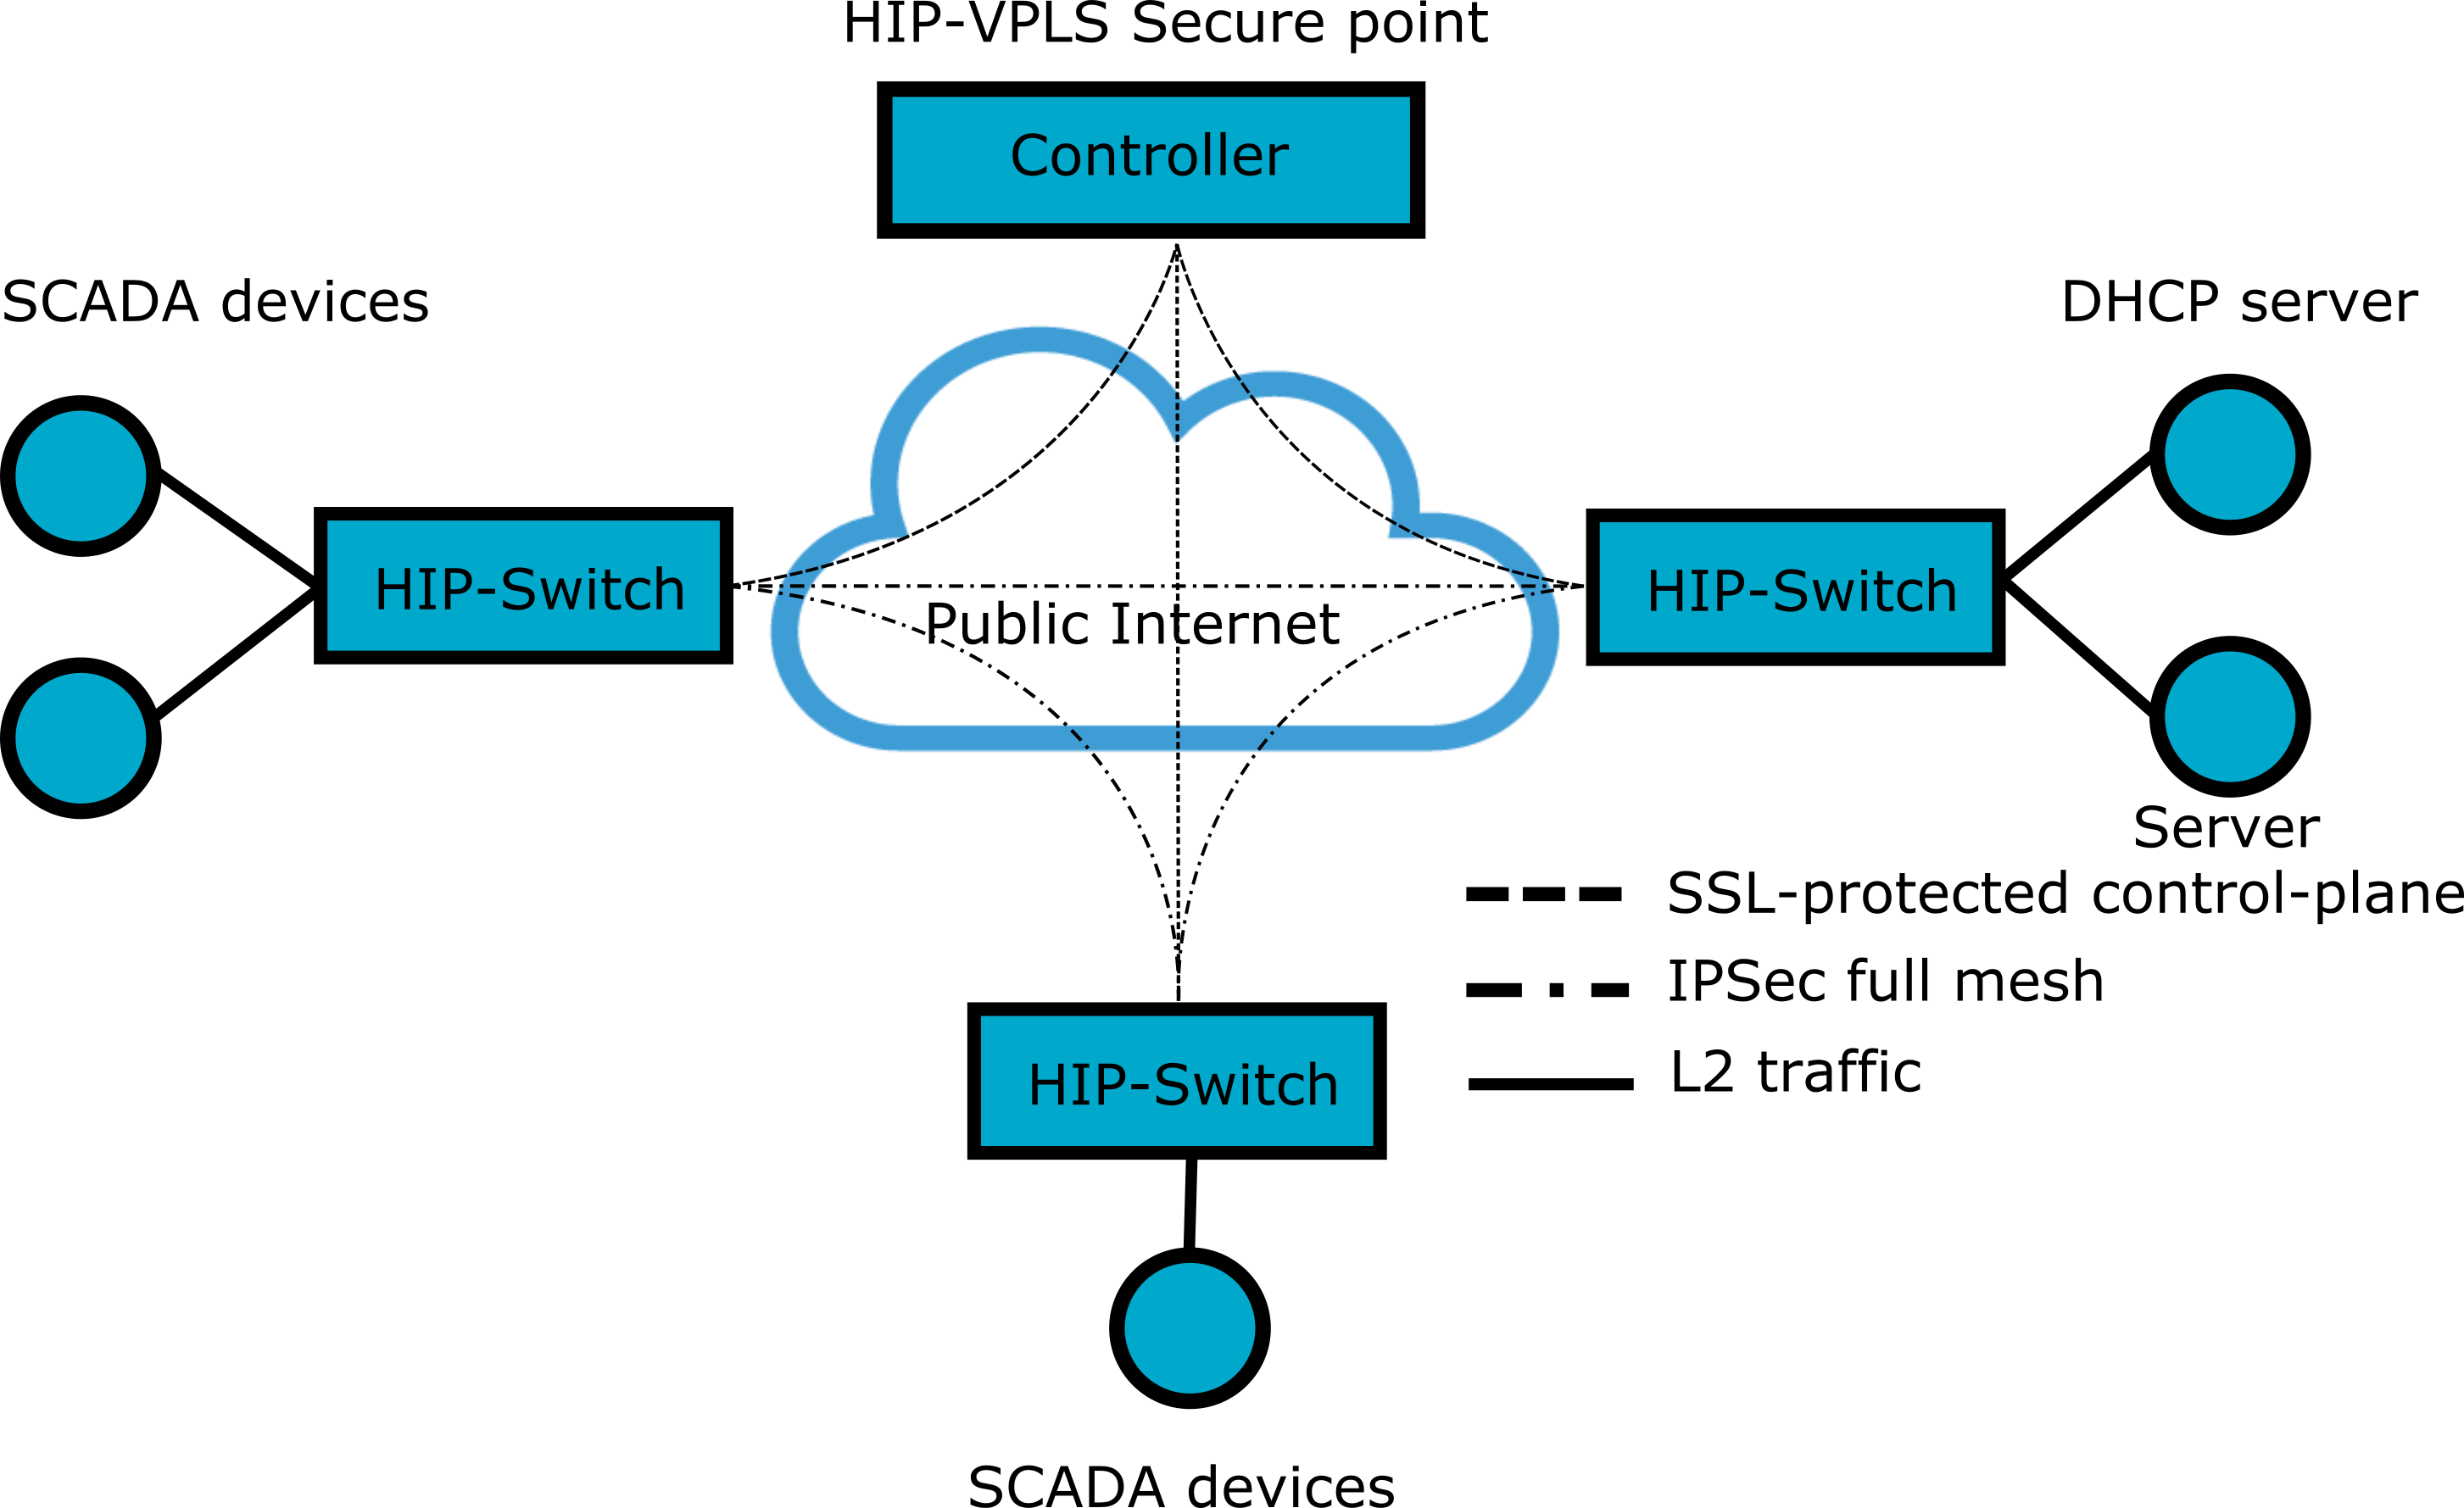
\includegraphics[width=0.9\textwidth]{graphics/arch.png}
\caption{System architecture}
\label{fig:architecture}
\end{figure} 

Although we did not implement traffic shaper feature in our HIP-switches and HIP 
controller, we believe that it is still valuable for the future work.
For example, different hosts can be served differently (have more bandwidth)
than some other hosts by using traffic shaping. For example, if some hosts in HIP-VPLS 
network send delay sensitive traffic, for example, curtain rules can be configured 
on HIP controller to give needed advantage over other hosts in the network. We leave 
this for the future discussions and work.
    
\chapter{Proof-of-a-concept implementation}
In this chapter, we are going to discuss the proof of a concept, or prototype,
implementation of the HIP-VPLS (we are going to discuss how HIP-switches and 
controller were implemented). In our work we have used the Python language 
as it offers simplicity at the cost of extra CPU cycles to do the job.

The experimental test-bed is shown in Figure~\ref{fig:testbed}.

\begin{figure}[h!]
\centering
\includegraphics[width=0.9\textwidth]{graphics/testbed.png}
\caption{Testbed setup}
\label{fig:testbed}
\end{figure}    

Our prototype implementation consists of roughly 10K lines of code. Overall,
the deployed architecture is shown in Figure~\ref{fig:architecture}. The communication
between the HIP-VPLS switches is secured with HIP and IPSec protocols. The communication
with the HIP-VPLS controller is secured with SSL protocol. We have chosen HIP protocol
to secure the data plane traffic as it does not rely on the TCP, hence reduces the 
wasted bandwidth. 

The communication with the HIP-VPLS controller is authenticated using self-signed
certificates. In addition client authenticates itself to the controller using HMAC
and preshared master secret. The format of the control packets can be looked up in the 
HIP controller source code found in our Git repository~\cite{controller-impl}. 

To deploy the system, we have prepared the bash script. Overall the deployment is trivial.
The only things that are needed to change is the master secret and MySQL password. Otherwise,
the administrator needs to execute the following commands in the server's console (note, 
we have tested on Ubuntu 22.04.2 LTS). So, to deploy the system run the following (note,
that one needs to change the MySQL password in deploy.sh and config.py files (for
both controller and configurator)):

\begin{verbatim}
$ git clonse https://github.com/strangebit-io/hip-vpls-controller.git
$ cd hip-vpls-controller/deployment
$ sudo bash deploy.sh
\end{verbatim}

After HIP controller and configurator were deployed, one needs to deploy the HIP switch code
on NanoPI R2S (remember you need to copy the certchain.pem - self-signed certificates
and change the master secret to match the one specified for HIP controller. Also, 
administrator needs to change the public, routable in the Internet, IP address in the 
configuration and specify the switch name):


\begin{verbatim}
$ https://github.com/strangebit-io/hip-vpls-hw-with-controller.git
$ cd hip-vpls-hw-with-controller/
$ sudo bash deployment/deploy.sh
\end{verbatim}

Once important aspect. The clocks on NanoPI R2S needs to be set to UTC and should be
synchronized with the controller (otherwise, certificate verification will fail during
the SSL handshake).

Once everything is set open the browser and open the location http://192.168.1.3:10000/ (or, 
whatever the IP address of the HIP controller node). You should see the following screen (
see Figure~\ref{fig:login}). The credentials can be found in schema.sql file in database folder. 

\begin{figure}[h!]
\centering
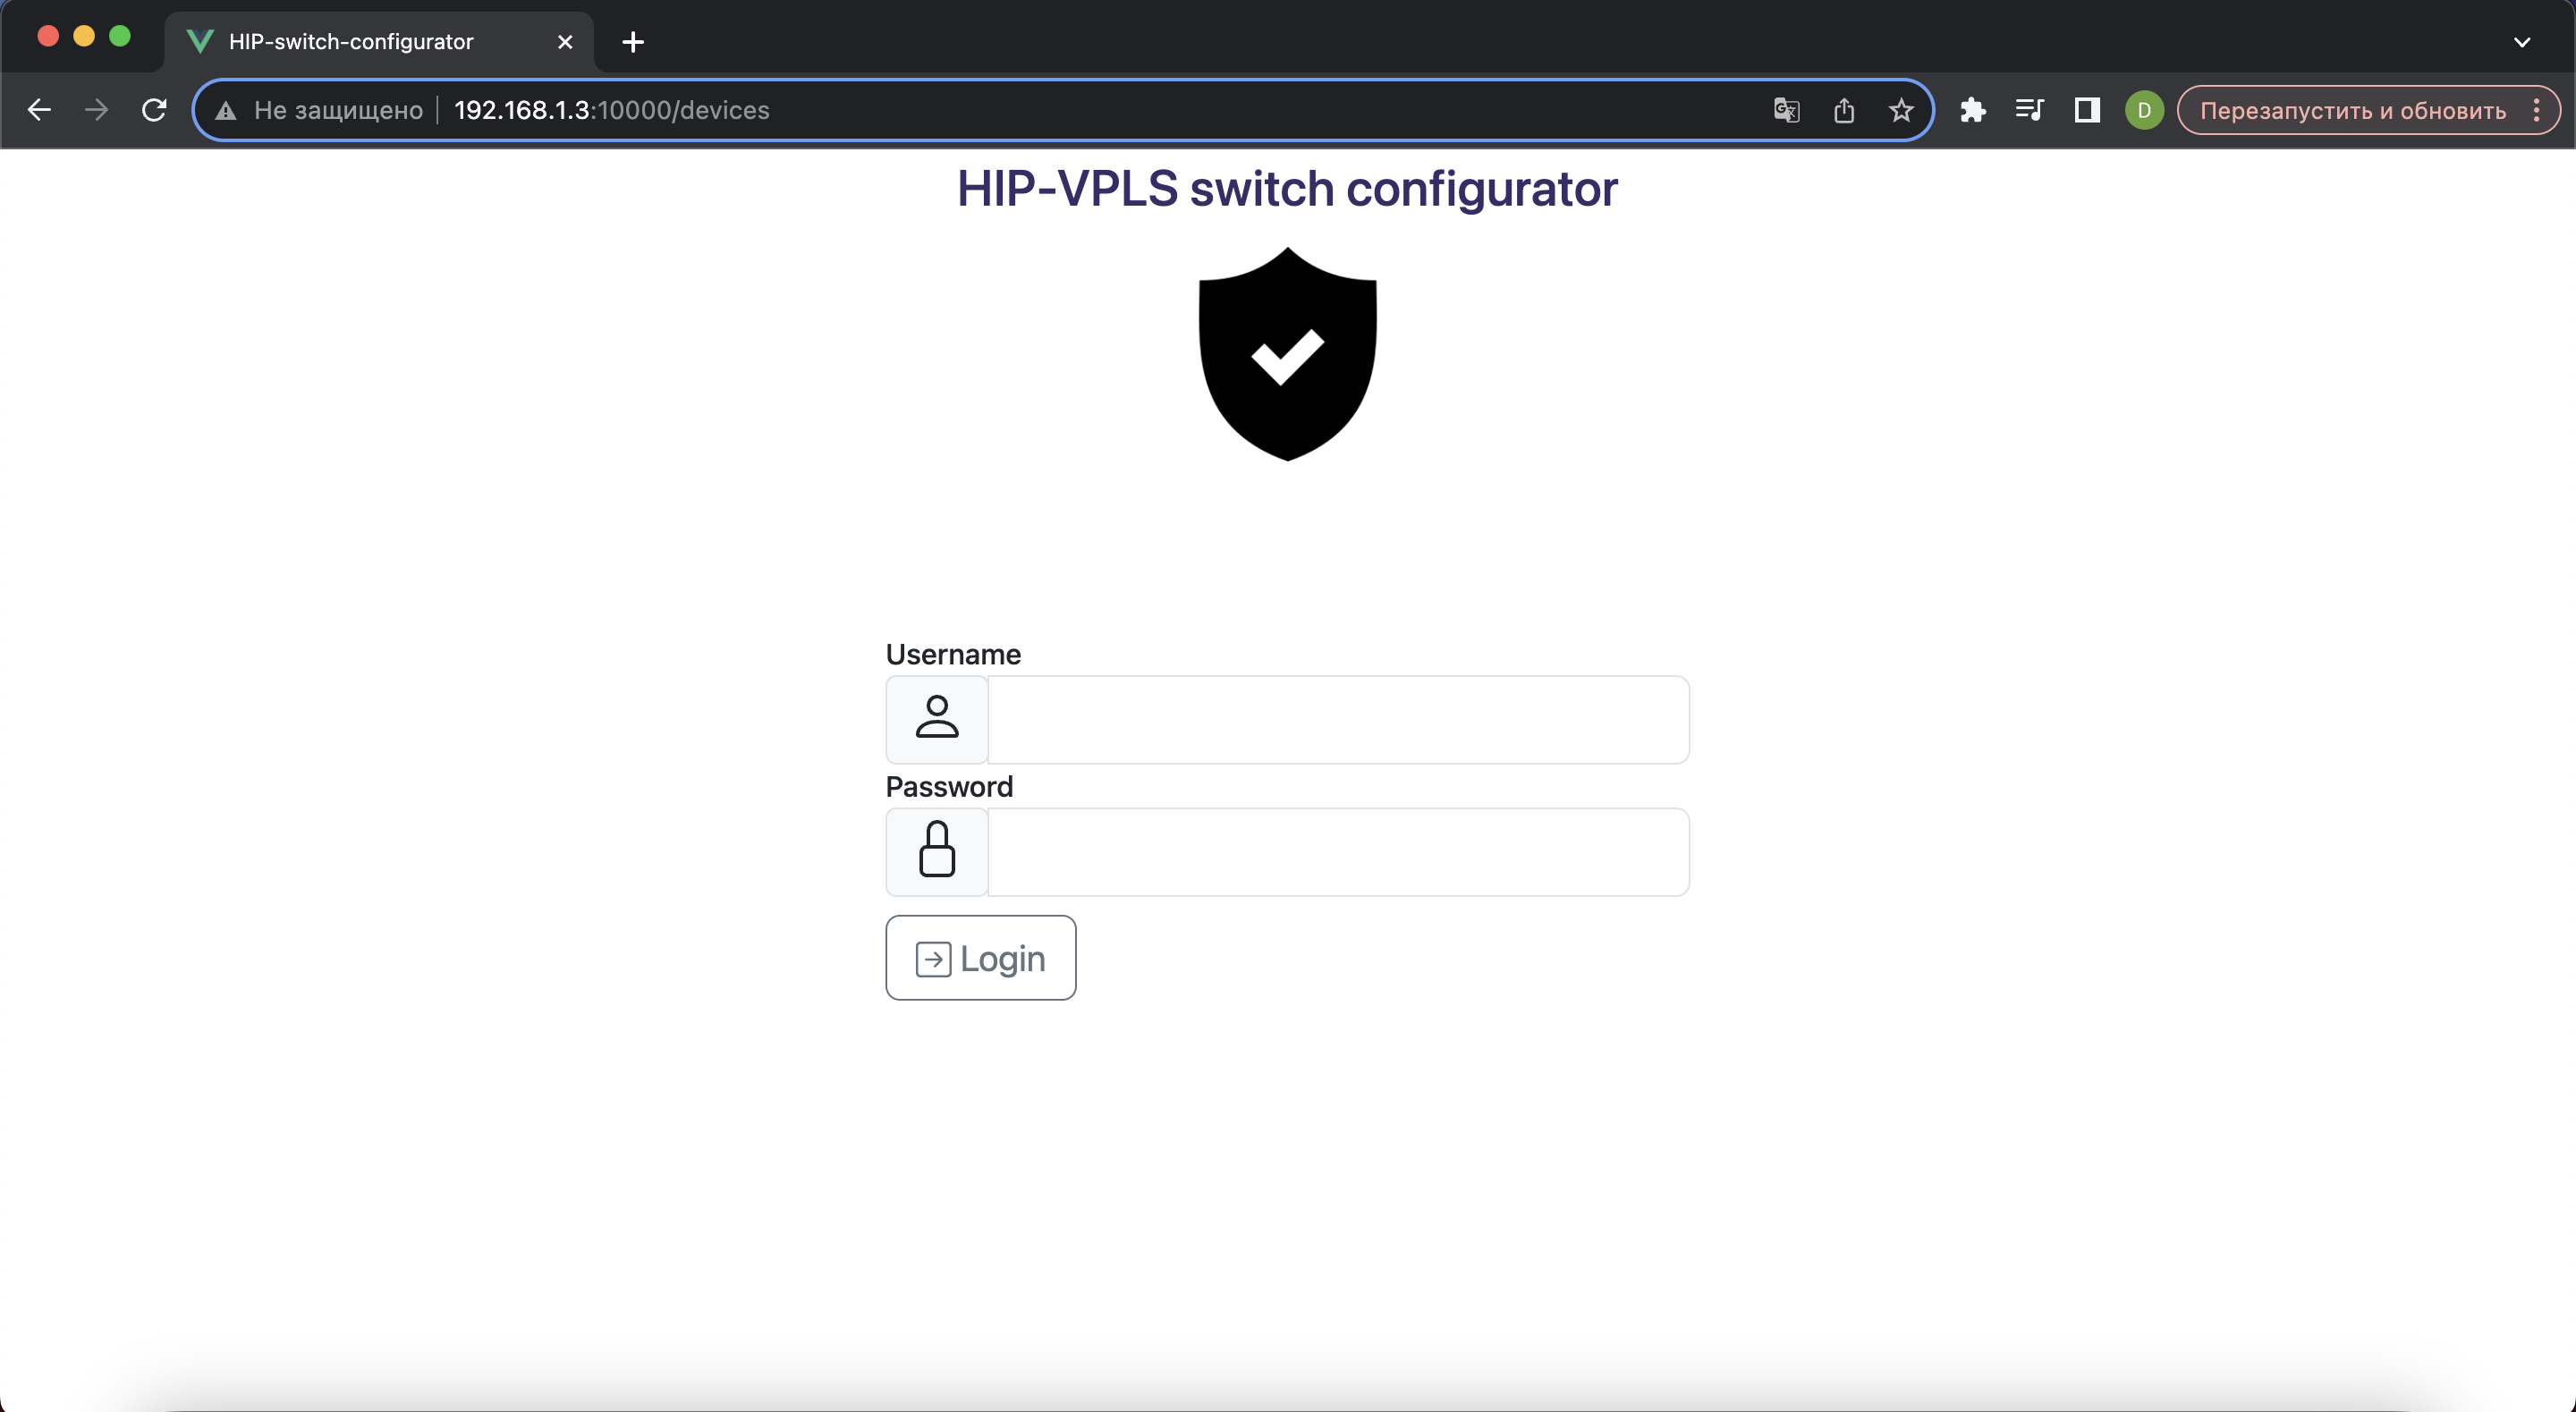
\includegraphics[width=0.9\textwidth]{graphics/login_screen.png}
\caption{Prototype: login screen}
\label{fig:login}
\end{figure}

After successful login the device status page will open. Here, all registered (registration is 
performed automatically) HIP switches will appear. You can check the status, HIT and IP of the 
switches.

\begin{figure}[h!]
\centering
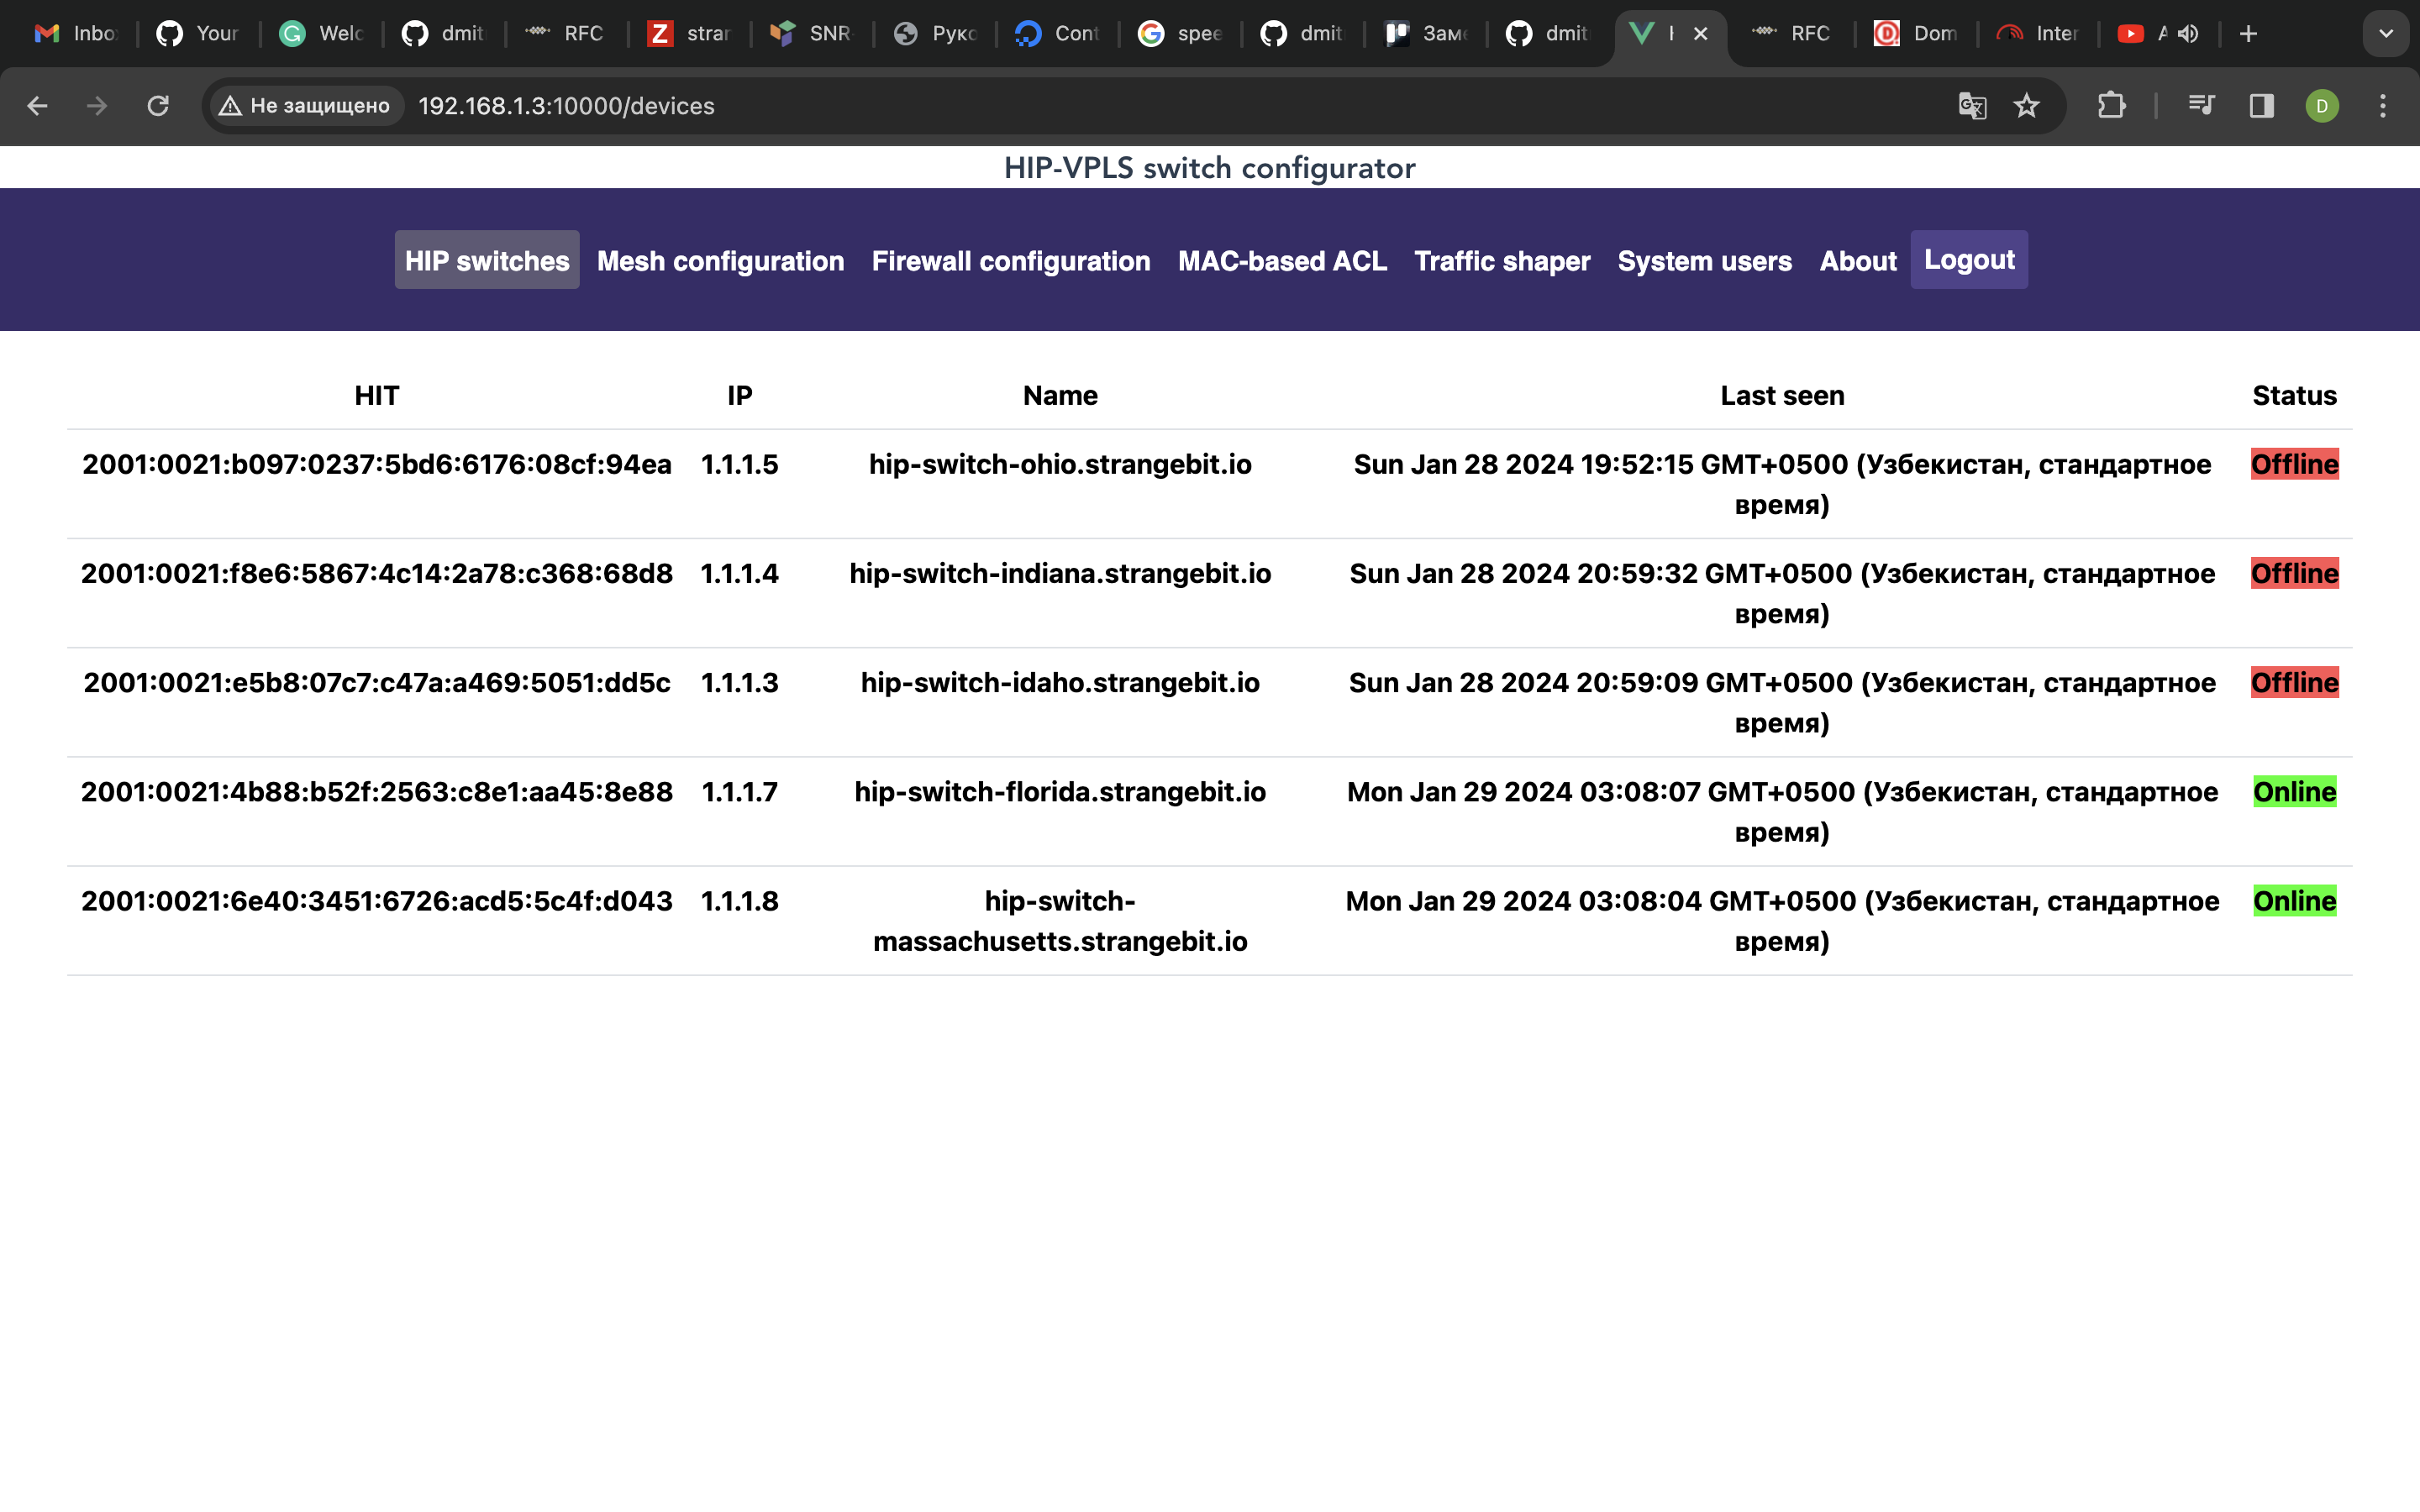
\includegraphics[width=0.9\textwidth]{graphics/devices.png}
\caption{Prototype: devices status information}
\label{fig:devices}
\end{figure}

Next, one needs to configure the mesh for distributed network. In our setup we simply listed
all possible pair of HIP-switches. That is the typical configuration option. For example, see
Figure~\ref{fig:mesh}.

\begin{figure}[h!]
\centering
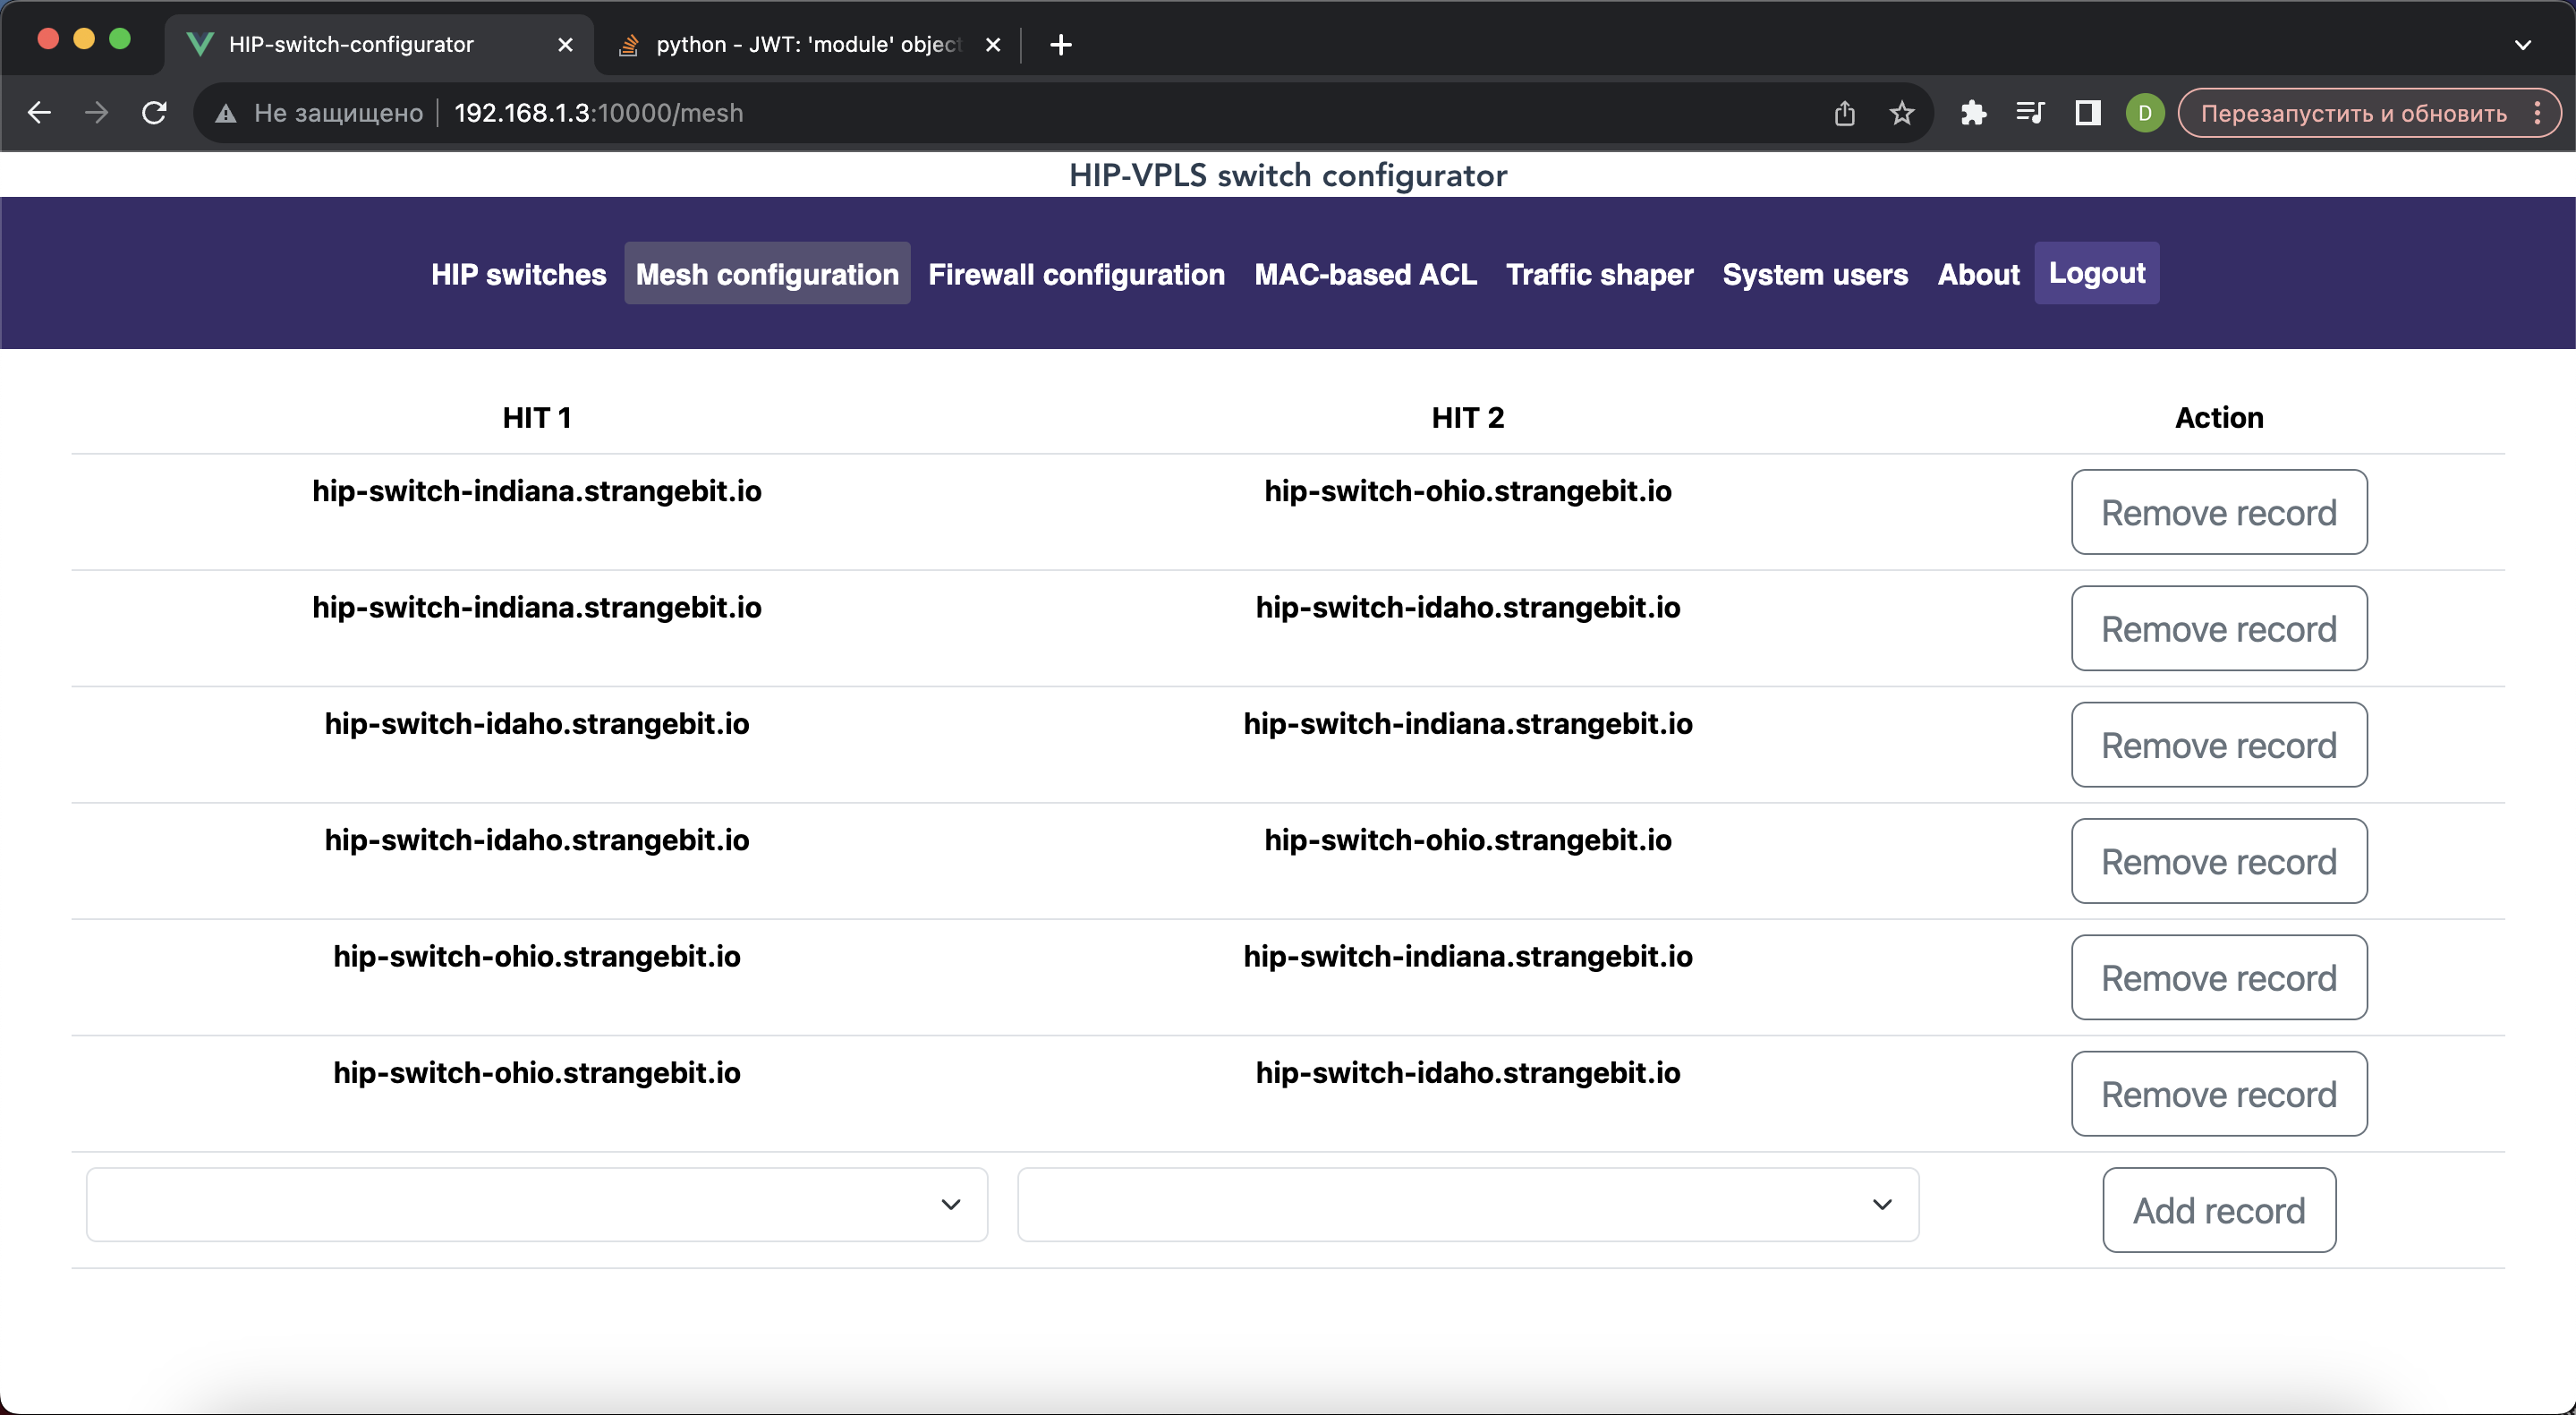
\includegraphics[width=0.9\textwidth]{graphics/mesh.png}
\caption{Prototype: mesh configuration}
\label{fig:mesh}
\end{figure}

Then we need to specify the HIP firewall rules. This operation should be done on firewall tab. 
See Figure~\ref{fig:mesh}. Again, a typical setup should have all pairs of HITS.

\begin{figure}[h!]
\centering
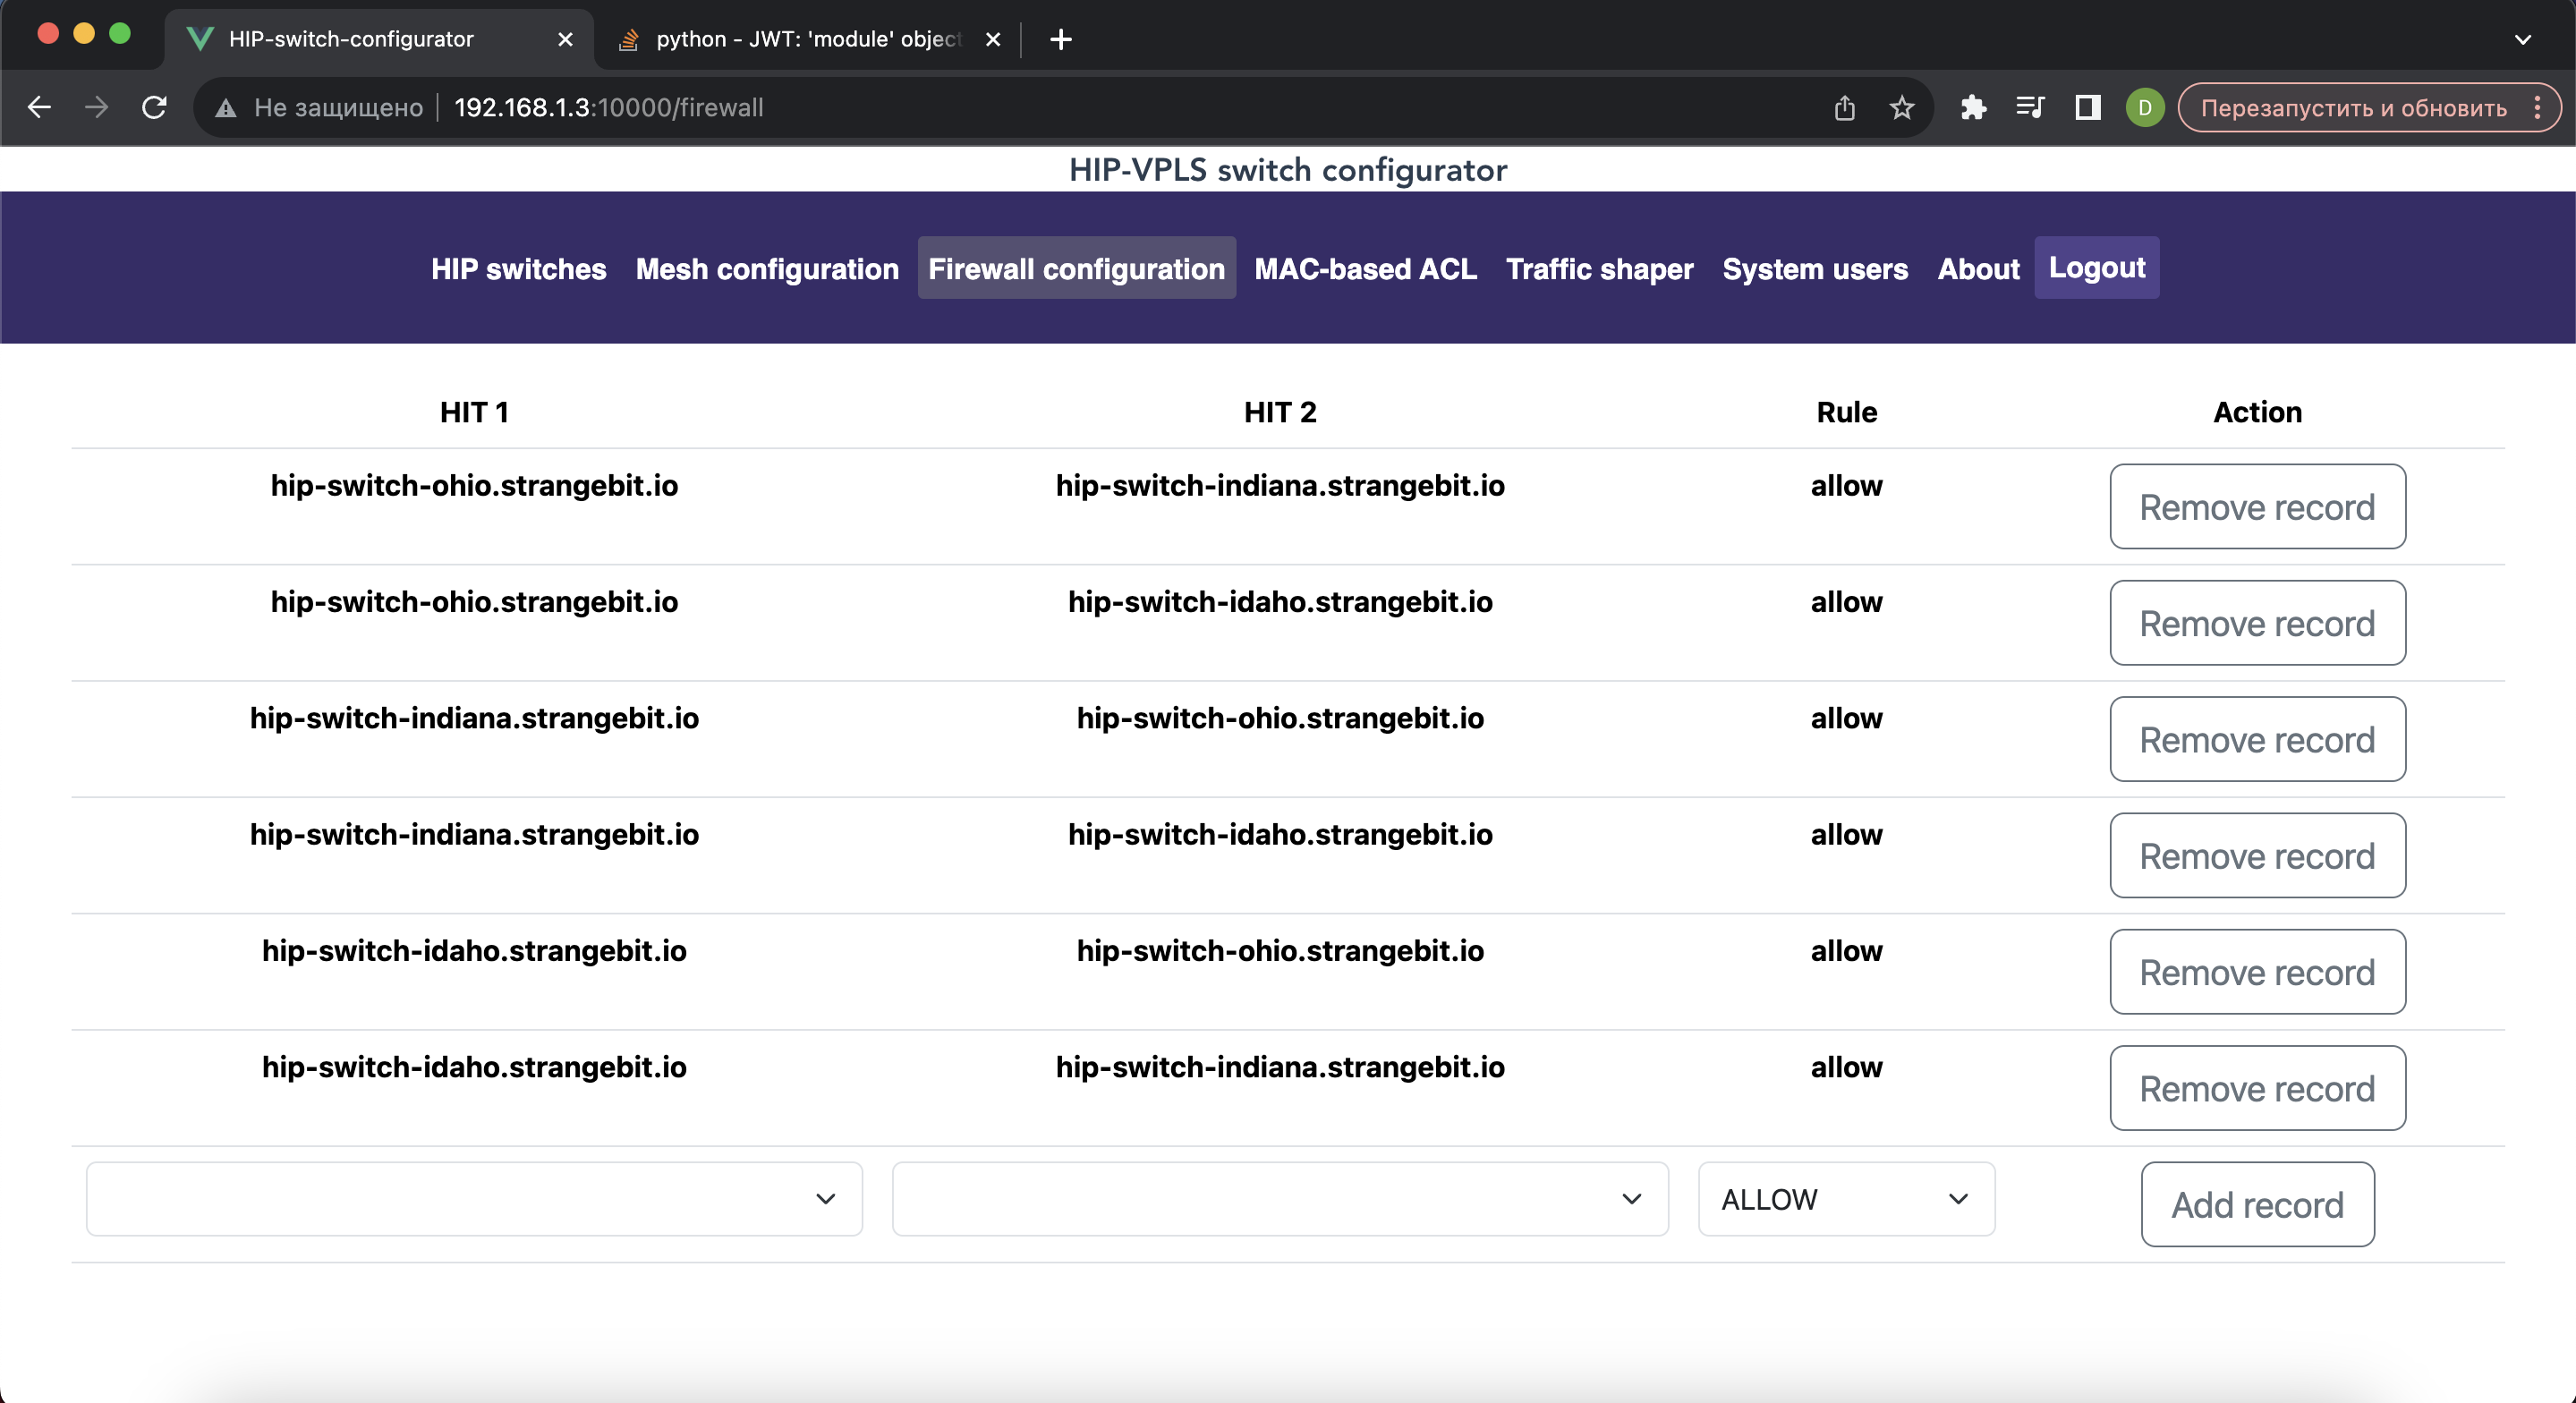
\includegraphics[width=0.9\textwidth]{graphics/HIP-firewall.png}
\caption{Prototype: HIP firewall}
\label{fig:mesh}
\end{figure}

The final step is to configure MAC address-based access control (see Figure~\ref{fig:mac}). 
Here we need to specify (in outgoing direction) necessary MAC address pairs of hosts in the network.
Remember this step need to be completed for each HIP switch separately.

\begin{figure}[h!]
\centering
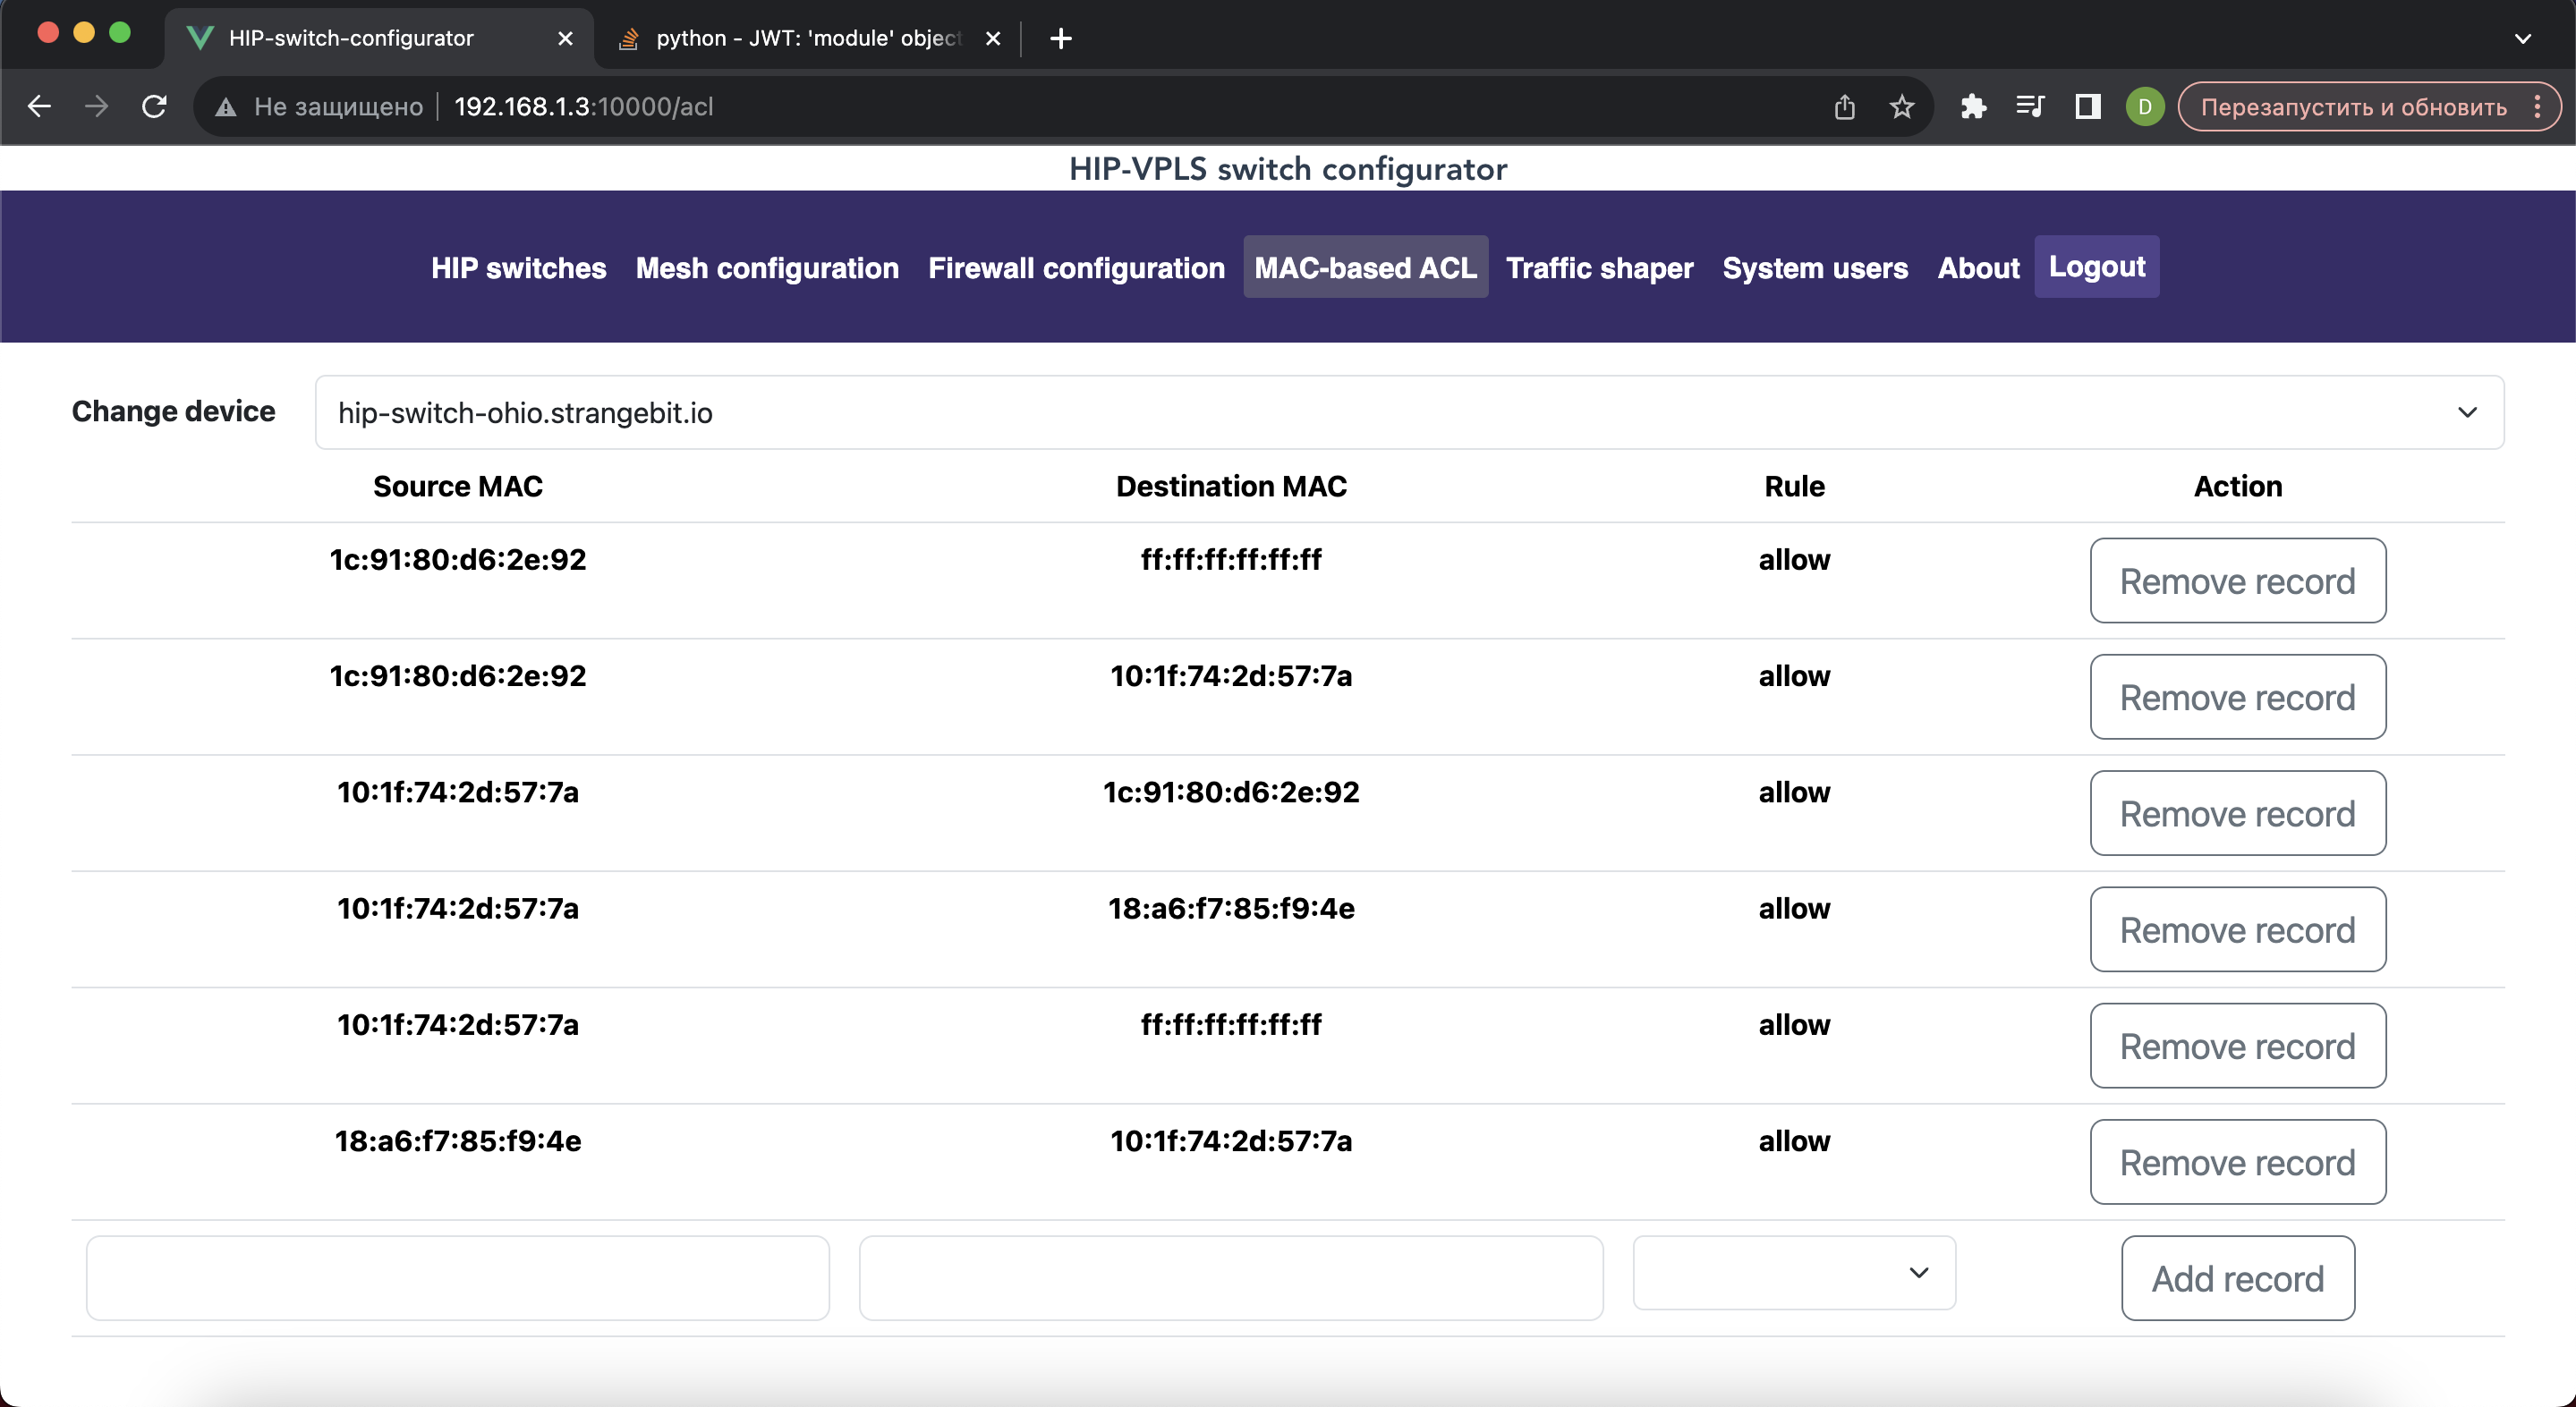
\includegraphics[width=0.9\textwidth]{graphics/MAC-ACL.png}
\caption{Prototype: MAC address based access control lists}
\label{fig:mac}
\end{figure}

%\begin{figure}[h!]
%\centering
%
\includegraphics[width=0.9\textwidth]{graphics/reg_packet.png}
%\caption{Registration packet}
%\label{fig:reg_packet}
%\end{figure}

%\section{Accelerating AES with the hardware}

Overall, we were not satisfied with the HIP switches. We were observing roughly $120 Kbits/s$ throughput
using IPerf tool. So we have tried to improve the performance by implementing in C++ and assembly language
AES256 cryptographic algorithm. Luckily, NanoPI R2S chip (ARM Cortex 53) supports AES256 instruction set.
We have cross compiled the library and used it in our HIP switch implementation. The results for AES256 
encryption is shown in Figure~\ref{fig:aes}. The performance of AES256 implemented with special CPU 
instructions was 10 times better. Thus, our preliminary experiments showed that we can achieve roughly 
$2.3 Mbits/s$ throughput between pair of hosts.

\begin{figure}[h!]
\centering
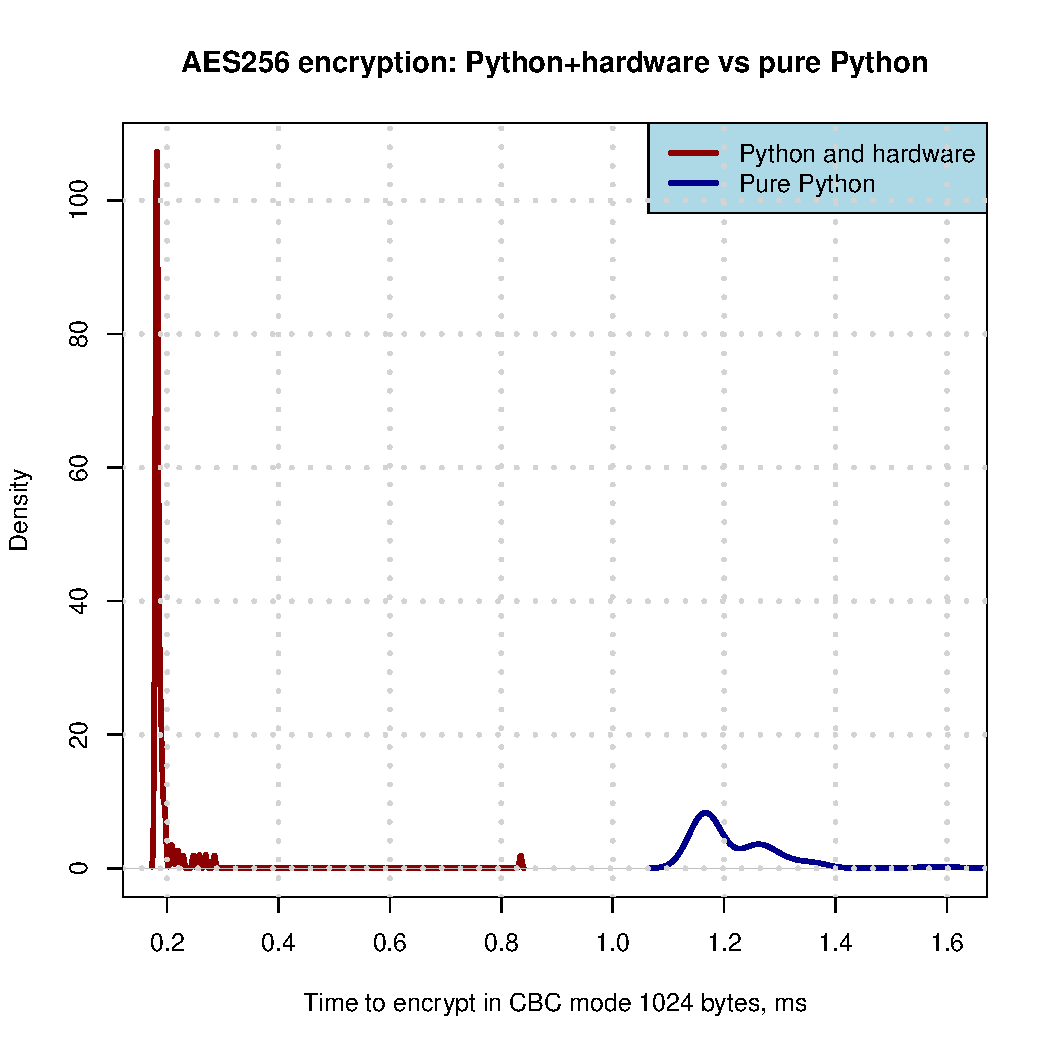
\includegraphics[width=0.9\textwidth]{graphics/AES.pdf}
\caption{AES encryption performance}
\label{fig:aes}
\end{figure}





